\clearpage
\section{Робот Balancing Arm}
\subsection{Обзор робота}
Балансировочный рычаг TETRIX Prime -- это сборка
, которая демонстрирует, как можно применять концепции управления, преподаваемые
на инженерных курсах. Сама рукоятка
вращается серводвигателем и балансирует
мяч в положении, указанном пользователем (т.е.
заданное значение). Сервопривод управляется
ПИД-регулятором с замкнутым контуром.
Алгоритм, реализован в LabVIEW. Данные
обратной связи - это положение мяча, которое собирается
с инфракрасного (ИК) датчика. Если мяч находится вне
положения, разница между заданным значением
и данными о положении с ИК-датчика (т.е. ошибка)
будет рассчитан, и цикл PID будет корректировать его с течением времени.

\subsection{Описание робота}
Балансировочный рычаг вращается серводвигателем, который получает данные о положении PWM.
Положение мяча измеряется инфракрасным датчиком (ИК), который вводит данные по аналоговой линии.
Пользователь задает заданное значение положения на передней панели LabVIEW VI.
Система постепенно перемещает мяч в нужное положение с помощью ПИД-регулятора.
После сборки пользователь должен откалибровать рычаг, указав положение сервопривода, при котором рычаг
параллелен земле.
Перед каждым использованием пользователь также должен откалибровать контроллер, чтобы распознать минимальные и максимальные края
рычага.
Коэффициенты усиления PID настраиваются автоматически, не требуя ввода пользователем.

\newpage
\subsection{Сборка робота}
\begin{figure}[h]
    \begin{subfigure}[b]{0.45\textwidth}
        \centering
        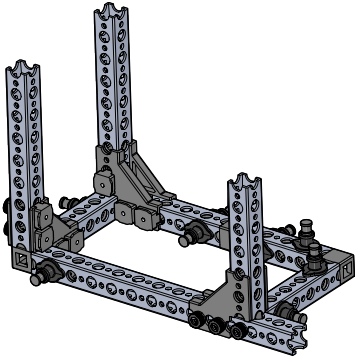
\includegraphics[width=0.7\textwidth]{fig/assembly/2.1.png}
        \caption*{Шаг 1}
    \end{subfigure}
    \begin{subfigure}[b]{0.45\textwidth}
        \centering
        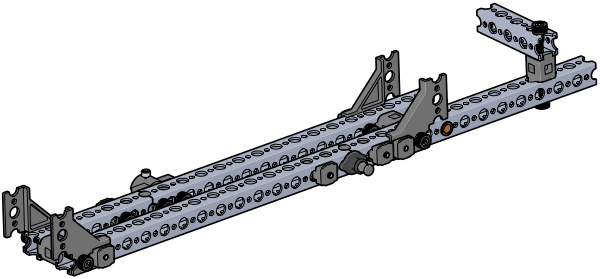
\includegraphics[width=0.7\textwidth]{fig/assembly/2.2.png}
        \caption*{Шаг 2}
    \end{subfigure}
    \begin{subfigure}[b]{0.45\textwidth}
        \centering
        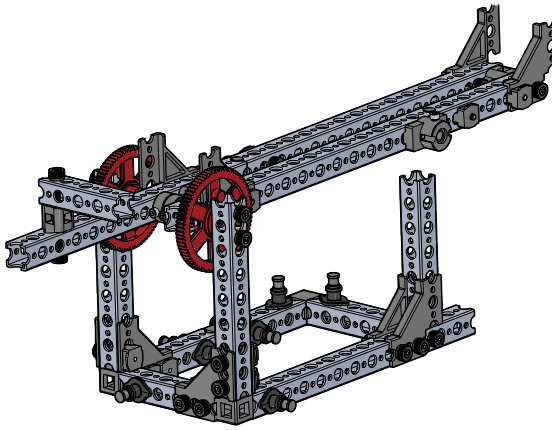
\includegraphics[width=0.7\textwidth]{fig/assembly/2.3.png}
        \caption*{Шаг 3}
    \end{subfigure}
    \begin{subfigure}[b]{0.45\textwidth}
        \centering
        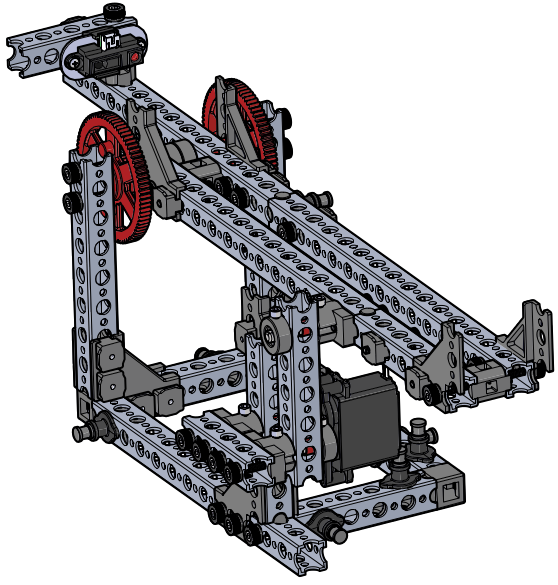
\includegraphics[width=0.7\textwidth]{fig/assembly/2.4.png}
        \caption*{Шаг 4}
    \end{subfigure}
    \begin{subfigure}[b]{0.45\textwidth}
        \centering
        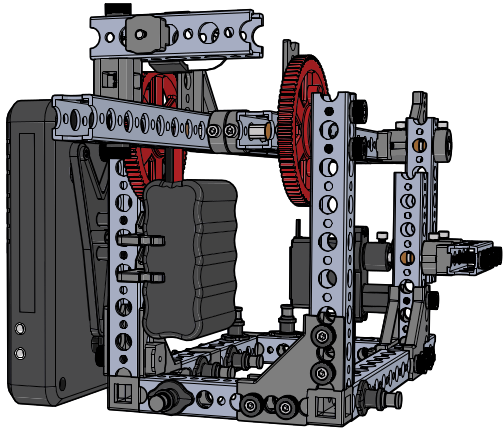
\includegraphics[width=0.7\textwidth]{fig/assembly/2.5.png}
        \caption*{Шаг 5}
    \end{subfigure}
    \begin{subfigure}[b]{0.45\textwidth}
        \flushright
        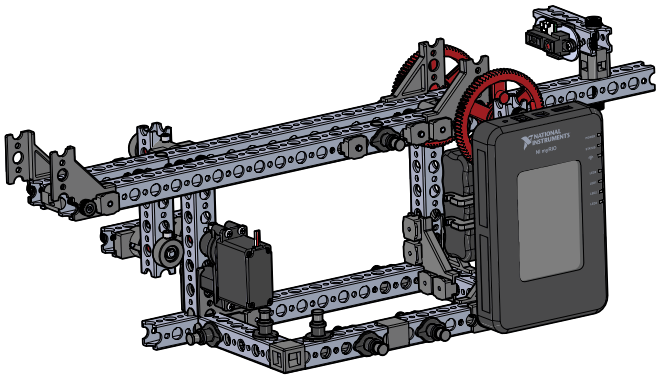
\includegraphics[width=0.7\textwidth]{fig/assembly/2.6.png}
        \caption*{Шаг 6}
    \end{subfigure}
\end{figure}

\newpage
\subsection{Подключение робота}
Подключение робота представлено на рисунке \ref{2connect}.
\begin{figure}[h]
    \centering
    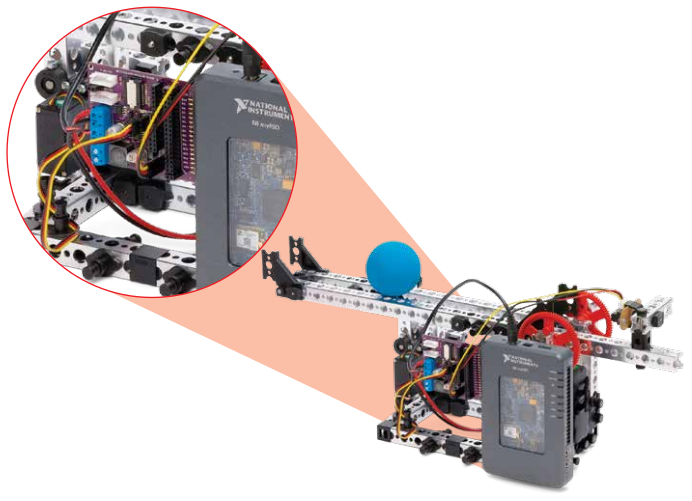
\includegraphics[width=0.7\textwidth]{fig/assembly/2.7.png}
    \caption{Подключение двигателей и периферии}
    \label{2connect}
\end{figure}

\subsection{Испытание робота}
Балансировочный рычаг и один стандартный серводвигатель являются установкой и приводом соответственно. Датчик является
датчиком ИК диапазона и обеспечивает сигнал обратной связи о местоположении мяча относительно датчика, по которому мы можем вычислить
смещение от заданного значения. Команды поступают в систему управления через главный компьютер через
команды передней панели, отправляемые по USB соединению Ethernet на myRIO, на котором размещен код ПИД-регулятора.
Управляющая программа робота представлена на рисунке \ref{2prog}.
\begin{figure}[h]
    \centering
    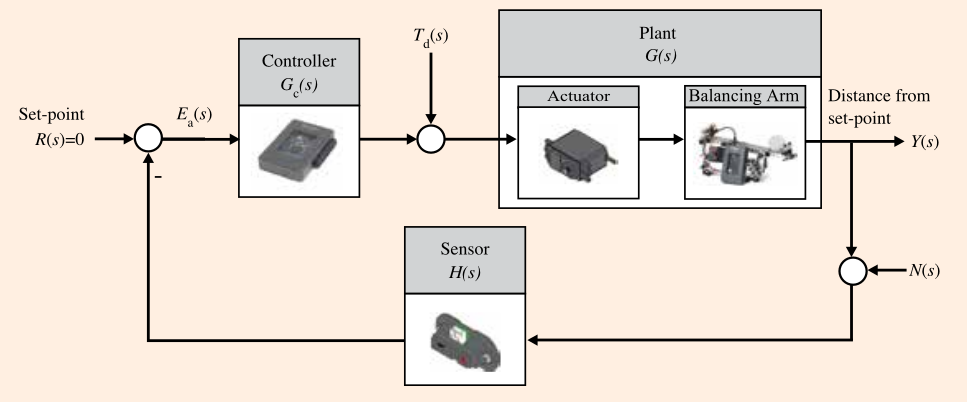
\includegraphics[width=0.7\textwidth]{fig/assembly/2.8.png}
    \caption{Управляющая программа робота}
    \label{2prog}
\end{figure}

%\subsection{Устранение неисправностей}
%\begin{itemize}
%    \item Убедитесь, что стол, за которым вы работаете, ровный и неподвижный
%    \item Убедитесь, что и myRIO, и аккумулятор надежно закреплены в системе, так как их вес способствует устойчивости
%    \item Убедитесь, что ИК-датчик расположен по центру направляющей
%    \item Если электрождвигатели вращаются в неправильном направлении, поменяйте полярность подключения двигателей или активируйте их реверс в программе управления.
%\end{itemize}